\documentclass[11pt,a4paper,english]{article}

%\usepackage{fullpage}
\usepackage{a4wide}
\usepackage[utf8]{inputenc}
\usepackage{sidecap}
\usepackage{babel}
\usepackage{amsmath}
\usepackage{amssymb}
\usepackage{verbatim}
\usepackage{units}
\usepackage{wrapfig}
\usepackage{setspace}
\usepackage{url}
%\usepackage{slashbox}
\usepackage{listing}
\usepackage{xcolor}
\usepackage{textcomp}
\usepackage{graphicx}
\usepackage{caption}
\usepackage{subcaption}
\usepackage{multirow}
\usepackage[colorlinks=false,pdfborder={0 0 0}]{hyperref}
\usepackage{cleveref}
\usepackage{float}
\usepackage{mathtools}
\usepackage{listings}
\usepackage{color}
\usepackage{cases}
\usepackage[T1]{fontenc}
\usepackage{slashbox}
\usepackage{todonotes}
\usepackage{algorithm2e}
\allowdisplaybreaks
\crefname{lstlisting}{listing}{listings}
%\usepackage[framed,numbered,autolinebreaks,useliterate]{mcode}

%\lstset{
%	captionpos =	b,
%	frame =	single
%}
\definecolor{dkgreen}{rgb}{0,0.6,0}
\definecolor{gray}{rgb}{0.5,0.5,0.5}
\definecolor{mauve}{rgb}{0.58,0,0.82}
\lstset{frame=tb,
  language=Matlab,
  aboveskip=3mm,
  belowskip=3mm,
  showstringspaces=false,
  columns=flexible,
  basicstyle={\small\ttfamily},
  numbers=none,
  numberstyle=\tiny\color{gray},
  keywordstyle=\color{blue},
  commentstyle=\color{dkgreen},
  stringstyle=\color{mauve},
  breaklines=true,
  breakatwhitespace=true
  tabsize=3
}

\crefname{algocf}{alg.}{algs.}
\Crefname{algocf}{Algorithm}{Algorithms}

\providecommand{\SetAlgoLined}{\SetLine}
\providecommand{\DontPrintSemicolon}{\dontprintsemicolon}
\DeclarePairedDelimiter{\abs}{\lvert}{\rvert}
\DeclarePairedDelimiter{\norm}{\lVert}{\rVert}
\DeclarePairedDelimiter{\ceil}{\lceil}{\rceil}
\DeclarePairedDelimiter{\floor}{\lfloor}{\rfloor}
\DeclarePairedDelimiter{\setN}{\{}{\}}

\newcommand{\bs}{\boldsymbol}
\newcommand{\pr}[1]{\text{Pr}\left (#1 \right)}
\renewcommand\arraystretch{1.0}

\title{Advanced algorithms and data structures\\
       Assignment 1: Minimum-cost Flow}

\author{
  Philip Munksgaard\\
    University of Copenhagen\\
    \texttt{pmunksgaard@gmail.com}
    \and
	Malte Stær Nissen\\
    University of Copenhagen\\
	  \texttt{malte.nissen@gmail.com}
    \and
  Jacob Daniel Kirstejn Hansen\\
    University of Copenhagen\\
    \texttt{jkirstejn@gmail.com}
}

\date{\today}

\begin{document}

\maketitle

\tableofcontents
\clearpage

\section{Exercise 1: $b$-flow}
 
\subsection{Figure 1(a)}
 
The following is a \emph{b}-flow for the graph in Figure 1(a):
 
\begin{align*}
  f(v_1, v_3) &= 4 \\
  f(v_2, v_1) &= 5 \\
  f(v_2, v_5) &= 1 \\
  f(v_3, v_2) &= 4 \\
  f(v_3, v_4) &= 3 \\
  f(v_4, v_5) &= 1 \\
  f(v_5, v_1) &= 2 \\
  f(v_5, v_3) &= 7 \\
\end{align*}
 
This holds because; for each vertex, the sum of the incoming flow minus the   
sum of the outgoing flow is exactly the demand of that vertex.                

\subsection{Figure 1(b)}
 
There exists no \emph{b}-flow for the graph in Figure 1(b). This is best seen 
by inspecting vertex $v_4$ that has a negative demand of $-2$, meaning it     
needs to send 2 units away from the vertex, as negative capacities are not    
defined. However, $v_4$ only has ingoing edges and is therefore not able to   
meet its demands, meaning that a \emph{b}-flow does not exist.                

\begin{comment}
There exists no \emph{b}-flow for the graph in Figure 1(b). $v_1$ in has a    
demand of $3$, and since the only incoming edge is the one from $v_2$ with    
capacity $3$, we use that edge to fulfill $v_1$s demand. $v_2$ has a demand   
of $1$, but as the only incoming edge is the one from $v_3$ only has capacity 
$2$, and because we have to send a flow of $3$ to $v_1$, $v_2$ cannot fulfill 
its demands.                                                                  
\end{comment}

\section{Exercise 2: Minimum-cost flow problem}
 
We assign variable names to all the edges in Figure 1(a):
 
\begin{align*}
 x_1 :=& v_1v_3 \\
 x_2 :=& v_1v_4 \\
 x_3 :=& v_2v_1 \\
 x_4 :=& v_2v_4 \\
 x_5 :=& v_2v_5 \\
 x_6 :=& v_3v_2 \\
 x_7 :=& v_3v_4 \\
 x_8 :=& v_4v_5 \\
 x_9 :=& v_5v_1 \\
 x_{10} :=& v_5v_3 \\
\end{align*}
 
We then want to minimize                                                      
$x_1+2x_2+3x_3+4x_4+5x_5+6x_6+7x_7+8x_8+9x_9+10x_{10}$ with the following     
constraints:                                                                  

\begin{table}[H]
   \begin{tabular}{rrrrrrrrrrrr}
   $x_1$  & ~      & ~      & ~      & ~      & ~      & ~      & ~      & ~      & ~         & $\leq$ & $ 4$ \\
   ~      & $x_2$  & ~      & ~      & ~      & ~      & ~      & ~      & ~      & ~         & $\leq $ & $1$ \\
   ~      & ~      & $x_3$  & ~      & ~      & ~      & ~      & ~      & ~      & ~         & $\leq$ & $ 5$ \\
   ~      & ~      & ~      & $x_4$  & ~      & ~      & ~      & ~      & ~      & ~         & $\leq$ & $ 2$ \\
   ~      & ~      & ~      & ~      & $x_5$  & ~      & ~      & ~      & ~      & ~         & $\leq$ & $ 3$ \\
   ~      & ~      & ~      & ~      & ~      & $x_6$  & ~      & ~      & ~      & ~         & $\leq$ & $4$  \\
   ~      & ~      & ~      & ~      & ~      & ~      & $x_7$  & ~      & ~      & ~         & $\leq$ & $ 3$ \\
   ~      & ~      & ~      & ~      & ~      & ~      & ~      & $x_8$  & ~      & ~         & $\leq $ & $2$ \\
   ~      & ~      & ~      & ~      & ~      & ~      & ~      & ~      & $x_9$  & ~         & $\leq $ & $6$ \\
   ~      & ~      & ~      & ~      & ~      & ~      & ~      & ~      & ~      & $x_{10}$  & $\leq $ & $7$ \\
   $-x_1$ & $-x_2$ & $+x_3$ & ~      & ~      & ~      & ~      & ~      & $+x_9$ & ~         & $=$ & $ 3$    \\
   ~      & ~      & $-x_3$ & $-x_4$ & $-x_5$ & $+x_6$ & ~      & ~      & ~      & ~         & $=$ & $-2$    \\
   $x_1$  & ~      & ~      & ~      & ~      & $+x_6$ & $-x_7$ & ~      & ~      & $+x_{10}$ & $=$ & $4$     \\
   ~      & $x_2$  & ~      & $+x_4$ & ~      & ~      & $+x_7$ & $-x_8$ & ~      & ~         & $=$ & $2$     \\
   ~      & ~      & ~      & ~      & $x_5$  & ~      & ~      & $+x_8$ & $-x_9$ & $-x_{10}$ & $=$ & $-7$    \\
   $x_1,$ & $x_2,$ & $x_3,$ & $x_4,$ & $x_5,$ & $x_6,$ & $x_7,$ & $x_8,$ & $x_9,$ & $x_{10}$  & $\geq$ & $ 0$ \\
   \end{tabular}
\end{table}

We notice the linear programming formulation is not on standard form,         
so to fix this we convert the objective function into a maximisation          
problem by multiplying $-1$ on each side, meaning we have to maximize:        
$-x_1-2x_2-3x_3-4x_4-5x_5-6x_6-7x_7-8x_8-9x_9-10x_{10}$.                      

We then convert all the equality constraints into inequality constraints,     
using the fact that $A \geq B, A \leq B \Leftrightarrow A = B$. However then  
we obtain $\geq$-inequalities which are not allowed in the standard form,     
so we convert these to $\leq$-inequalities by multiplying each side of the    
inequality with $-1$. The standard form of the linear programming formulation 
then looks as follows.                                                        

\begin{table}[H]
   \begin{tabular}{rrrrrrrrrrrr}
   $x_1$  & ~      & ~      & ~      & ~      & ~      & ~      & ~      & ~      & ~         & $\leq$ & $4$  \\
   ~      & $x_2$  & ~      & ~      & ~      & ~      & ~      & ~      & ~      & ~         & $\leq$ & $1$  \\
   ~      & ~      & $x_3$  & ~      & ~      & ~      & ~      & ~      & ~      & ~         & $\leq$ & $5$  \\
   ~      & ~      & ~      & $x_4$  & ~      & ~      & ~      & ~      & ~      & ~         & $\leq$ & $2$  \\
   ~      & ~      & ~      & ~      & $x_5$  & ~      & ~      & ~      & ~      & ~         & $\leq$ & $3$  \\
   ~      & ~      & ~      & ~      & ~      & $x_6$  & ~      & ~      & ~      & ~         & $\leq$ & $4$  \\
   ~      & ~      & ~      & ~      & ~      & ~      & $x_7$  & ~      & ~      & ~         & $\leq$ & $3$  \\
   ~      & ~      & ~      & ~      & ~      & ~      & ~      & $x_8$  & ~      & ~         & $\leq$ & $2$  \\
   ~      & ~      & ~      & ~      & ~      & ~      & ~      & ~      & $x_9$  & ~         & $\leq$ & $6$  \\
   ~      & ~      & ~      & ~      & ~      & ~      & ~      & ~      & ~      & $x_{10}$  & $\leq$ & $7$  \\
   $-x_1$ & $-x_2$ & $+x_3$ & ~      & ~      & ~      & ~      & ~      & $+x_9$ & ~         & $\leq$ & $3$  \\
   $x_1$  & $+x_2$ & $-x_3$ & ~      & ~      & ~      & ~      & ~      & $-x_9$ & ~         & $\leq$ & $-3$ \\
   ~      & ~      & $-x_3$ & $-x_4$ & $-x_5$ & $+x_6$ & ~      & ~      & ~      & ~         & $\leq$ & $-2$ \\
   ~      & ~      & $+x_3$ & $+x_4$ & $+x_5$ & $-x_6$ & ~      & ~      & ~      & ~         & $\leq$ & $2$  \\
   $x_1$  & ~      & ~      & ~      & ~      & $+x_6$ & $-x_7$ & ~      & ~      & $+x_{10}$ & $\leq$ & $4$  \\
   $-x_1$ & ~      & ~      & ~      & ~      & $-x_6$ & $+x_7$ & ~      & ~      & $-x_{10}$ & $\leq$ & $-4$ \\
   ~      & $x_2$  & ~      & $+x_4$ & ~      & ~      & $+x_7$ & $-x_8$ & ~      & ~         & $\leq$ & $2$  \\
   ~      & $-x_2$ & ~      & $-x_4$ & ~      & ~      & $-x_7$ & $+x_8$ & ~      & ~         & $\leq$ & $-2$ \\
   ~      & ~      & ~      & ~      & $x_5$  & ~      & ~      & $+x_8$ & $-x_9$ & $-x_{10}$ & $\leq$ & $-7$ \\
   ~      & ~      & ~      & ~      & $-x_5$ & ~      & ~      & $-x_8$ & $+x_9$ & $+x_{10}$ & $\leq$ & $7$  \\
   $x_1,$ & $x_2,$ & $x_3,$ & $x_4,$ & $x_5,$ & $x_6,$ & $x_7,$ & $x_8,$ & $x_9,$ & $x_{10}$  & $\geq$ & $0$  \\
   \end{tabular}
\end{table}

We can then formulate the dual problem of our linear programming form, which  
gives us the new objective function, that we wish to minimize: $4y_1 + y_2 +  
5y_3 + 2y_4 + 3y_5 + 4y_6 + 3y_7 + 2y_8 + 6y_9 + 7y_{10} + 3y_{11} - 3y_{12}  
- 2y_{13} + 2y_{14} + 4y_{15} - 4y_{16} + 2y_{17} - 2y_{18} - 7y_{19} +       
7y_{20}$.                                                                     

(table not complete, nearly done though)

\begin{table}[H]
  \begin{tabular}{rrrrrrrrrrrrrrrrrrrrr}
$y_1$  & ~     & ~     & ~     & ~     & ~     & ~     & ~     & ~    & ~     & $-y_1$ & $+y_1$ & ~     & ~     & $+y_1$ & $-y_1$ & ~     & ~      & ~ & ~  & $\geq$ & $-1$\\
~      & $y_2$ & ~     & ~     & ~     & ~     & ~     & ~     & ~    & ~     & $-y_2$ & $+y_2$ & ~     & ~     & ~     & ~      & $+y_2$ & $-y_2$ & ~ & ~  & $\geq$ & $-2$\\
~      & ~     & $y_3$ & ~     & ~     & ~     & ~     & ~     & ~    & ~     & $+y_3$ & $-y_3$ & $-y_3$ & $+y_3$ & ~   & ~      & ~     & ~     & ~ & ~    & $\geq$ & $-3$\\
~      & ~     & ~     & $y_4$ & ~     & ~     & ~     & ~     & ~    & ~     & ~      & ~      & $-y_4$ & $+y_4$ & ~   & ~      & $+y_4$& $-y_4$& ~ & ~    & $\geq$ & $-4$\\
~      & ~     & ~     & ~     & $y_5$ & ~     & ~     & ~     & ~    & ~     & ~      & ~      & $-y_5$ & $+y_5$ & ~   & ~ & ~   & ~     & $+y_5$ & $-y_5$ & $\geq$ & $-5$\\
~      & ~     & ~     & ~     & ~     & $y_6$ & ~     & ~     & ~    & ~     & ~      & ~      & ~     & ~     & ~     & ~      & ~     & ~     & ~ & ~    & $\geq$ & $-6$\\
~      & ~     & ~     & ~     & ~     & ~     & $y_7$ & ~     & ~    & ~     & ~      & ~      & ~     & ~     & ~     & ~      & ~     & ~     & ~ & ~    & $\geq$ & $-7$\\
~      & ~     & ~     & ~     & ~     & ~     & ~     & $y_8$ & ~    & ~     & ~      & ~      & ~     & ~     & ~     & ~      & ~     & ~     & ~ & ~    & $\geq$ & $-8$\\
~      & ~     & ~     & ~     & ~     & ~     & ~     & ~     & $y_9$& ~     & ~      & ~      & ~     & ~     & ~     & ~      & ~     & ~     & ~ & ~    & $\geq$ & $-9$\\
~      & ~     & ~     & ~     & ~     & ~     & ~     & ~     & ~    & $y_10$& ~      & ~      & ~     & ~     & ~     & ~      & ~     & ~     & ~ & ~    & $\geq$ & $-10$\\
  \end{tabular}
\end{table}

\section{Exercise 3: An application of MCFP: rectilinear planar embedding}

\subsection{}

Number of breakpoints total: 13

\begin{table}
    \begin{subtable}{0.5\textwidth}
        \centering
        \begin{tabular}{l | l | l}
            $f$ & $g$ & $z_{fg}$ \\ \hline
            a   & b & 0 \\
            a   & c & 0 \\
            a   & d & 0 \\
            a   & e & 0 \\
            b   & a & 2 \\
            b   & c & 1 \\
            b   & d & 1 \\
            b   & e & 0 \\
            c   & a & 1 \\
            c   & b & 1 \\
            c   & d & 0 \\
            c   & e & 0 \\
            d   & a & 0 \\
            d   & b & 1 \\
            d   & c & 0 \\
            d   & e & 2 \\
            e   & a & 4 \\
            e   & b & 0 \\
            e   & c & 0 \\
            e   & d & 0
        \end{tabular}
        \caption{All variables $z_{fg}$}
    \end{subtable}
    \begin{subtable}{0.5\textwidth}
        \centering
        \begin{tabular}{l | l | l}
            $v$ & $f$ & $x_{vf}$ \\ \hline
            $v_1$   & a & 0 \\
            $v_1$   & b & 1\\
            $v_1$   & c & 1 \\
            $v_2$   & b & 0 \\
            $v_2$   & c & 1 \\
            $v_2$   & d & 1 \\
            $v_3$   & a & 1 \\
            $v_3$   & c & 1 \\
            $v_3$   & d & 1 \\
            $v_3$   & e & 1 \\
            $v_4$   & d & -1 \\
            $v_4$   & e & 1 \\
            $v_5$   & a & 1 \\
            $v_5$   & e & -1 \\
            $v_6$   & a & 1 \\
            $v_6$   & b & 1 \\
            $v_6$   & d & 1 \\
            $v_6$   & e & 1 \\
            $v_7$   & a & 0 \\
            $v_7$   & e & 0
        \end{tabular}
        \caption{All variables $x_vf$}
    \end{subtable}
\end{table}

\begin{figure}[h]
    \centering
    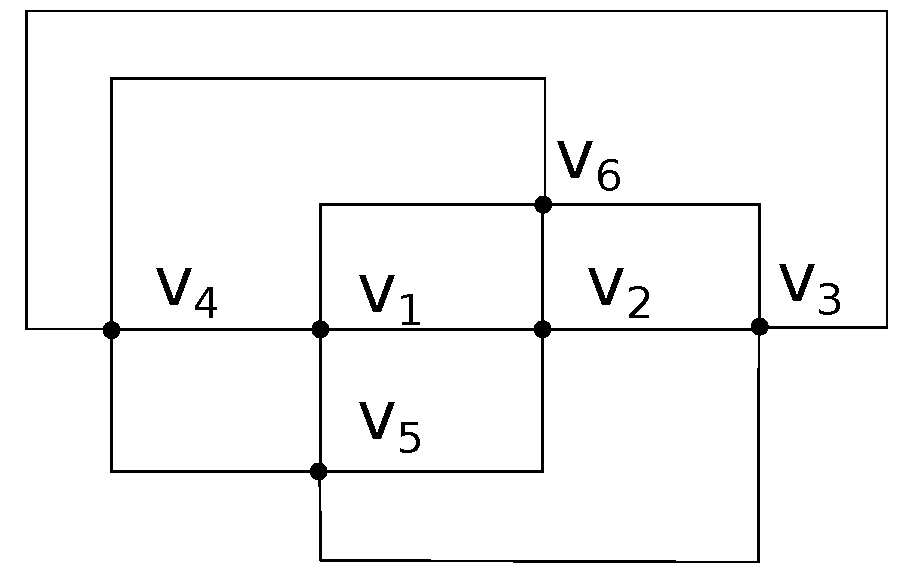
\includegraphics[width=0.5\textwidth]{rectilinear_layout.pdf}
    \caption{Rectilinear layout of graph}
\end{figure}

\subsection{}

\begin{align}
    b_f = \sum_{v \in V} x_{vf} + \sum_{g \in F} z_{fg} - z_{gf} = \begin{cases} -4 & f~\text{is external} \\ 4 & \text{otherwise}\end{cases}
\end{align}

\begin{align*}
    b_a &= \sum_{v \in V} x_{va} + \sum_{g \in F} z_{ag} - z_{ga},~~~ F = \{b,c,d,e\},~V = \{ v_1, v_3, v_5, v_6, v_7 \} \\
        &= 3 + (0 - 7) = -4 \\
    b_e &= \sum_{v \in V} x_{ve} + \sum_{g \in F} z_{eg} - z_{ge},~~~ F = \{a,d\},~V = \{ v_3, v_4, v_5, v_6, v_7 \} \\
        &= 2 + (4 - 2) = 4
\end{align*}

\subsection{}

As stated in the question we have assumed that no vertex in $G$ has degree
greater than 4. This assumption is necessary since we wouldn't be able to make
a rectilinear layout for vertices with degree greater than 4 since naturally
there are only 4 directions of horizontal/vertical edges (north, south, east
and west).

Furthermore we assume that no vertices in $G$ has degree lower than 2. If we
had vertices lower than 2 they wouldn't form a true corner on a face boundary.
Furthermore the vertex wouldn't be a true face boundary point since it would
be placed inside a face.

If a vertex $v$ has degree 2, it will only be a part of two faces $f_1$ and
$f_2$. When $x_{vf} = 0$ for one of the faces, the same will be the case for
the other face since this implies the two edges to lie on a straight line and
hence $\sum_f x_{vf} = 0$. If the two edges make a ``corner'', then $x_{vf}
= -1$ for one of the faces $f_1$ or $f_2$ and $x_{vf} = 1$ for the other and
hence we have $\sum_f x_{vf} = 0$ again.

If a vertex $v$ has degree 3, there will always have two of it's edges in a
straight line and hence contribution nothing to the sum. The third edge will
be perpendicular to both of the edges on the straight line and hence make a
inner turn on both of the faces that share the perpendicular edge. This will
contribute with 1 for each of the two faces and hence $\sum_f x_{vf} = 2$.

Given a vertex $v$ of degree 4, the vertex will always be part of 4 faces in
each of which the vertex will be creating an inner turn. This gives us $\sum_f
x_{vf} = 4$ and we have the following property of each vertex $v$:
\begin{align}
	\sum_f x_{vf} = \begin{cases}
				0 & \text{if}~v~\text{has degree 2} \\
				2 & \text{if}~v~\text{has degree 3} \\
				4 & \text{if}~v~\text{has degree 4} \\
			      \end{cases}
\end{align}

%Exercise 3.4 content
\subsection{}
 
Minimize $\sum_{f \in F, g \in F} z_{fg}$.
 
\begin{align*}
 \sum_{v \in V} x_{vf} + \sum_{g \in F} z_{fg} - z_{gf}\quad =& \quad \begin{cases} -4 & f~\text{is external} \\ 4 & \text{otherwise}\end{cases} \\
 \sum_f x_{vf} \quad =& \quad \begin{cases}
                                0 & \text{if}~v~\text{has degree 2} \\
                                2 & \text{if}~v~\text{has degree 3} \\
                                4 & \text{if}~v~\text{has degree 4} \\
                              \end{cases} \\
 z_{fg} \quad \geq& \quad 0 ~~\text{for all}~f,g \in F
\end{align*}
 
where $F$ is the set of faces in the graph.


%Exercise 3.5 content

\subsection{}

We want to translate the different properties of the rectilinear graph
$G = (V, E)$ into a graph $G'$ representing a minimum-cost-flow
problem. For simplicity we'll allow bidirectional edges; they can
easily be eliminated by introducing an intermediate vertex, so this
shouldn't be a problem.

To do this, each face in $G$ is translated into a vertex in the
minimum-cost-flow problem with demand $-4$ if the face is external and
$4$ otherwise. Vertices in $G'$ representing faces that share edges in
$G$ are connected bidirectionally to each other with edges that have $cost = 1,
capacity = \infty $.

Vertices in $G$ are also added to $G'$ as vertices with demand $0$ if
they have degree $2$, demand $2$ if they have degree $3$, and demand
$4$ if they have degree $4$. Now, the newly constructed vertices in
$G'$ representing vertices in $G$, are connected bidirectionally to
the vertices representing faces in $G$ for which they appear in the
boundary cycle. These edges are assigned capacities $1$ and cost $0$.

For two faces $a,b$ in $G$ and their corresponding vertices in $G'$
$v_a, v_b$, the flow of the edge going from the vertex $v_a$ to the
vertex $v_b$ represents to $z_{ba}$.

For a vertex $v_a$ in $G'$ representing face $a$ in $G$ and a vertex
$v'$ in $G'$ representing a vertex $v$ in $G$, the difference between
the flow going from $v'$ to $v_a$ represents $x_{vf}$.


\end{document}
